\lstdefinelanguage{Pseudo}{
	keywords={KLASSE, IMPORTIERE, OEFFENTLICH FUNKTION, ENDE, void},
	morecomment=[l]{//}
}

\lstdefinestyle{mystyle}{
    backgroundcolor=\color{backcolour},   
    commentstyle=\color{codegreen},
    keywordstyle=\color{magenta},
    numberstyle=\tiny\color{codegray},
    stringstyle=\color{codepurple},
    basicstyle=\ttfamily\footnotesize,
    breakatwhitespace=false,         
    breaklines=true,                 
    captionpos=b,                    
    keepspaces=true,                 
    numbers=left,                    
    numbersep=5pt,                  
    showspaces=false,                
    showstringspaces=false,
    showtabs=false,                  
    tabsize=2
}

\lstset{style=mystyle}

\chapter{Videospielentwicklung}
\label{chap:videospielentwicklung}

% Fortsetzen, Umschreiben

Jedes Videospiel hat seine eigenen Regeln, die der jeweilige Entwickler \"{u}ber eine bestimmte Programmiersprache entwickelt. So wurde beispielsweise das Arcade-Videospiel �Marble Madness� (1984) vom Entwicklerstudio Atari Games in C programmiert. Zuvor programmierte Atari Games ihre Spiele in Assemblersprache. Die heutigen Spielwelten werden von Entwicklern mithilfe einer Game-Engine entwickelt.


\section{Game-Engines}
\label{chap:game engines}

Mit dem Wachstum der Komplexit\"{a}t und Kosten von Videospielen entstanden Game-Engines. Eine Game-Engine ist eine Entwicklungsumgebung, in der Videospiele programmiert und zusammengestellt werden. 

Zum Zeitpunkt ihrer Entstehung wurden Game-Engines zwar nur f\"{u}r konkrete Videospiel-Serien geschrieben. So hat das Entwicklerstudio id Software ihre Videospiel-Serie Commander Keen (1990) als Game-Engine programmiert, was die Entwicklungszeit weiterer Commander Keen Spiele verk\"{u}rzte. Die Game-Engine wurde auch f\"{u}r andere Entwicklerstudios lizensiert, die \"{a}hnliche Videospiele wie Commander Keen entwickelten. Eine weitere bekanntere Game-Engine ist die Doom-Engine (id Tech), welche ebenfalls von id Software stammt und f\"{u}r das Videospiel Doom (1993) programmiert wurde. Die Doom-Engine hat dabei ein minimalistisches Ma\ss{} an Programmierbarkeit geboten. Benutzer konnten in der Game-Engine Daten in einem vorgegebenen Format hinzuf\"{u}gen. Die daraus entstandenen Spielwelten hatten dabei andere Layouts spielten sich aber wie Doom.

Heutzutage sind Game-Engines aber auch ein Sofware-Programm mit einer Kollektion an Modulen, die der Entwickler zur Entwicklung verschiedener Videospiel-Genres nutzt. Die Gr\"{o}\ss{}e der Game-Engine variiert nach der Anzahl an Funktionen, die durch bestimmte Module umgesetzt werden. Typische Funktionen sind das Rendern von Grafiken, die Verarbeitung von Eingaben \"{u}ber Eingabeger\"{a}te, Umsetzung von Physik und Kollisionen, Audio-Ausgabe und Netzwerk-Funktionen, die das Spielen mit anderen Spielern umsetzen. Zudem kann eine Game-Engine software development kits (SDKs) integrieren, die weitere Funktionen hinzuf\"{u}gen oder bereits bestehende Funktionen erweitern. Ein Beispiel f\"{u}r eine SDK ist Havok, die eine realistische Physik und Kollision umsetzt.

Game-Engines k\"{o}nnen f\"{u}r Entwickler entweder zug\"{a}nglich oder unzug\"{a}nglich sein. So entwickelte beispielsweise das deutsche Entwicklerstudio Crytek die Cryengine, die f\"{u}r andere Entwickler \"{u}ber Lizenzen zug\"{a}nglich ist. Demgegen\"{u}ber hat das Entwicklerstudio Dice mit der Frostbite Engine eine unzug\"{a}ngliche Game-Engine entwickelt. Die Entwicklung einer eigenen Game-Engine bei Indie-Entwicklerstudios ist schwer umsetzbar. Denn sie haben weniger Arbeitskr\"{a}fte als gro\ss{}e Entwicklerstudios und entwickeln Videospiele ohne finanzielle Unterst\"{u}tzung gr\"{o}\ss{}erer Unternehmen. Dadurch sind Indiestudios von m\"{o}glichst kosteng\"{u}nstigen sowie zug\"{a}nglichen Game-Engines abh\"{a}ngig. Unter zug\"{a}ngliche Game-Engines fallen unter anderem Unity, Unreal-Engine, Cry-Engine, RPGMaker, GameMaker und Godot.

Die Wahl oder Entwicklung einer bestimmten Game-Engine h\"{a}ngt von dem jeweiligen Genre und spezifischen Anforderungen des zu entwickelnden Videospiels ab. Einige Game-Engines konzentrieren sich auf ein spezifisches Genre. So konzentriert sich die idTech-Engine auf Shooter. W\"{a}hrend sich beispielsweise die RPGMaker-Engine auf das Genre der Rollenspiele spezialisiert, liegt der Fokus der Unreal-Engine auf der Entwicklung grafisch realistischer 3D-Videospiele.

%Programmiersprache erl\"{a}utern

\subsection{Godot}
\label{chap:godot}
Die \hyperref[chap:game engines]{Game-Engine} Godot ist seit 2014 in Entwicklung und open-source unter der MIT license verf\"{u}gbar. Sie erm\"{o}glicht die Entwicklung von Videospielen in 2D und 3D Umgebung. Bei Godot liegt der Fokus offiziell auf Desktop- und Mobile-Builds.\footnote{https://github.com/godotengine}

Die prim\"{a}re Programmiersprache in Godot ist GDScript, die explizit f\"{u}r Godot entwickelt wurde und der Programmiersprache Python syntaktisch \"{a}hnlich ist. Auch die Programmiersprache C# wird von Godot unterst\"{u}tzt. Dar\"{u}ber hinaus werden die Programmiersprachen D, Kotlin, Nim, Python und Rust bereits durch die Community \"{u}ber das GDNative System unterst\"{u}tzt. Offiziell f\"{o}rdert Godot \"{u}ber GDNative auch C und C++.\footnote{https://docs.godotengine.org/en/3.5/tutorials/scripting/gdnative/what_is_gdnative.html}

\subsection{Unity}
\label{chap:unity}

%Abo Satz erweitern?
Die Unity ist eine weitere \hyperref[chap:game engines]{Game-Engine}, die 2005 ver\"{o}ffentlicht wurde. Aktuell ist sie in einer kostenlosen Version erh\"{a}ltlich, erg\"{a}nzt durch verschiedene kostenpflichtige Abonnements f\"{u}r erweiterte Funktionen.\footnote{https://unity.com/de/products/compare-plans} Wie auch Godot erm\"{o}glicht Unity die Entwicklung von Videospielen in 2D und 3D. Unity unterst\"{u}tzt die Entwicklung von Videospielen f\"{u}r Desktop-, Mobile, Konsolen- und Virtual-Reality-Plattformen.

Unitys prim\"{a}re Programmiersprache ist C#. Unity unterst\"{u}tzt auch visuelle Programmierl\"{o}sungen wie Bolt, durch die wenig oder gar nicht programmieren werden muss.\footnote{https://docs.unity3d.com/2019.3/Documentation/Manual/VisualScripting.html}

\subsection{Unreal-Engine}
\label{chap:unreal-engine}

Die Unreal-Engine wurde mit dem FPS Unreal 1998 ver\"{o}ffentlicht und von Epic Games entwickelt. Die Unreal-Engine ist kostenlos erh\"{a}ltlich. Dabei fallen Lizenzgeb\"{u}hren von 5\%erst ab einem Bruttoproduktumsatz von 1 Million USD an.\footnote{https://www.unrealengine.com/de/license} Durch die \hyperref[chap:game engines]{Game-Engine} ist es m\"{o}glich, Videospiele in 2D und 3D Umgebung zu entwickeln. Sie fokussiert sich dabei auf die 3D Umgebung und 3D Grafik und ist vielseitig portabel, unter anderem auf Desktop-, Mobile, Konsolen- und Virtual-Reality-Plattformen. 
%Editor weiter erl\"{a}utern
Prim\"{a}r wird C++ als Programmiersprache genutzt. Python ist ausschlie\ss{}lich f\"{u}r die Werkzeuge im Editor vorgesehen und kann nicht f\"{u}r die Spiellogik verwendet werden.\footnote{https://dev.epicgames.com/documentation/en-us/unreal-engine/unreal-engine-programming-and-scripting}


\section{Entwicklung eines GameObjects}
\label{chap:komponenten}

GameObjects sind Objekte der Spielwelt und werden \"{u}ber ihre Komponenten gesteuert. Eine Komponente kann einem GameObject beispielsweise die Funktion geben, die Spielumgebung wahrzunehmen und mit ihr zu interagieren. Eine Komponente wird \"{u}ber Skripte realisiert. \hyperref[chap:game engines]{Game-Engines} wie Godot, Unity und Unreal-Engine setzen bereits vordefinierte Komponenten mit ihren eigenen Methoden um. Meistens sind Komponenten in ihrer Funktion zu simpel, sodass ihre Skripte modifiziert oder erweitert werden m\"{u}ssen. Diese Skripte werden mit einer Programmiersprache angepasst, die, je nach Game-Engine, variieren kann.

Die folgende Abbildung veranschaulicht den grundlegenden Aufbau eines solchen Skripts in Pseudocode.

\begin{lstlisting}[language=Pseudo, caption={Aufbau eines Komponenten Skripts}]
IMPORTIERE Game-Engine Module

KLASSE Komponente

	//Deklaration und Initialisierung von Variablen
	
	FUNKTION ready() :void
		//Fuer die Initialisierung genutzt
	ENDE ready()

	FUNKTION update() :void
		//Wird jedes Frame aufgerufen
	ENDE ready()
	
	//Weitere Funktionen

ENDE KLASSE Komponente

\end{lstlisting}

\section{Game-AI}
\label{chap:game-ai}

Ein GameObject kann unter anderem ein Agent der Spielwelt sein und wird in diesem Fall als Non-Player-Character (NPC) bezeichnet. Im Gegensatz zu der Spielfigur werden NPCs von dem Computer gesteuert. Die Aufgabe der NPCs ist es, die Spielwelt immersiver zu gestalten. Daf\"{u}r nutzen Spieleentwickler akademische Forschungen aus dem Bereich der AI, um solche Algorithmen zu entwickeln, die NPCs der Spielwelt ein menschlicheres oder tierischeres Verhalten verleihen. Je nach Narrativ k\"{o}nnen NPCs mit der Spielfigur freundlich, neutral oder feindlich interagieren. Ein Beispiel f\"{u}r feindliche NPCs sind die Geister in Pac-Man. Darin versuchen sie, die Spielfigur in der Spielwelt zu fangen.

Die Game-AI wird \"{u}ber \hyperref[chap:game-objects]{Komponenten} realisiert und l\"{a}sst sich in drei Bereiche unterteilen: Bewegung (\textit{Movement}), Entscheidungsfindung (\textit{Decision making}) und Strategie (\textit{Strategy}). W\"{a}hrend Bewegung und Entscheidungsfindung sich auf einzelne NPCs beziehen, wird die Strategie-AI auf Gruppen von NPCs (\textit{Group AI}) angewendet. Nicht alle Videospiele ben\"{o}tigen alle der drei genannten Bereiche. So ben\"{o}tigt Schach keine Game-AI f\"{u}r Bewegung oder Entscheidungsfindung, sondern ausschlie\ss{}lich f\"{u}r Strategie.

Der Bereich der Bewegungs-AI arbeitet haupts\"{a}chlich mit Algorithmen, die daf\"{u}r sorgen, dass ein NPC von einer Position zu der N\"{a}chsten gelangt, Hindernissen ausweicht oder den optimalen Pfad zu einem Ziel findet.

Eine Strategie-AI sorgt f\"{u}r die Koordination einer ganzen Gruppe von NPCs. Sie soll dabei die Entscheidungsfindung der NPCs beeinflussen. Beispielsweise hat die Strategie-AI des FPS Half-Life die feindlichen NPCs dazu gebracht, die Spielerfigur zu flankieren.

\begin{figure}[h]
  \centering
  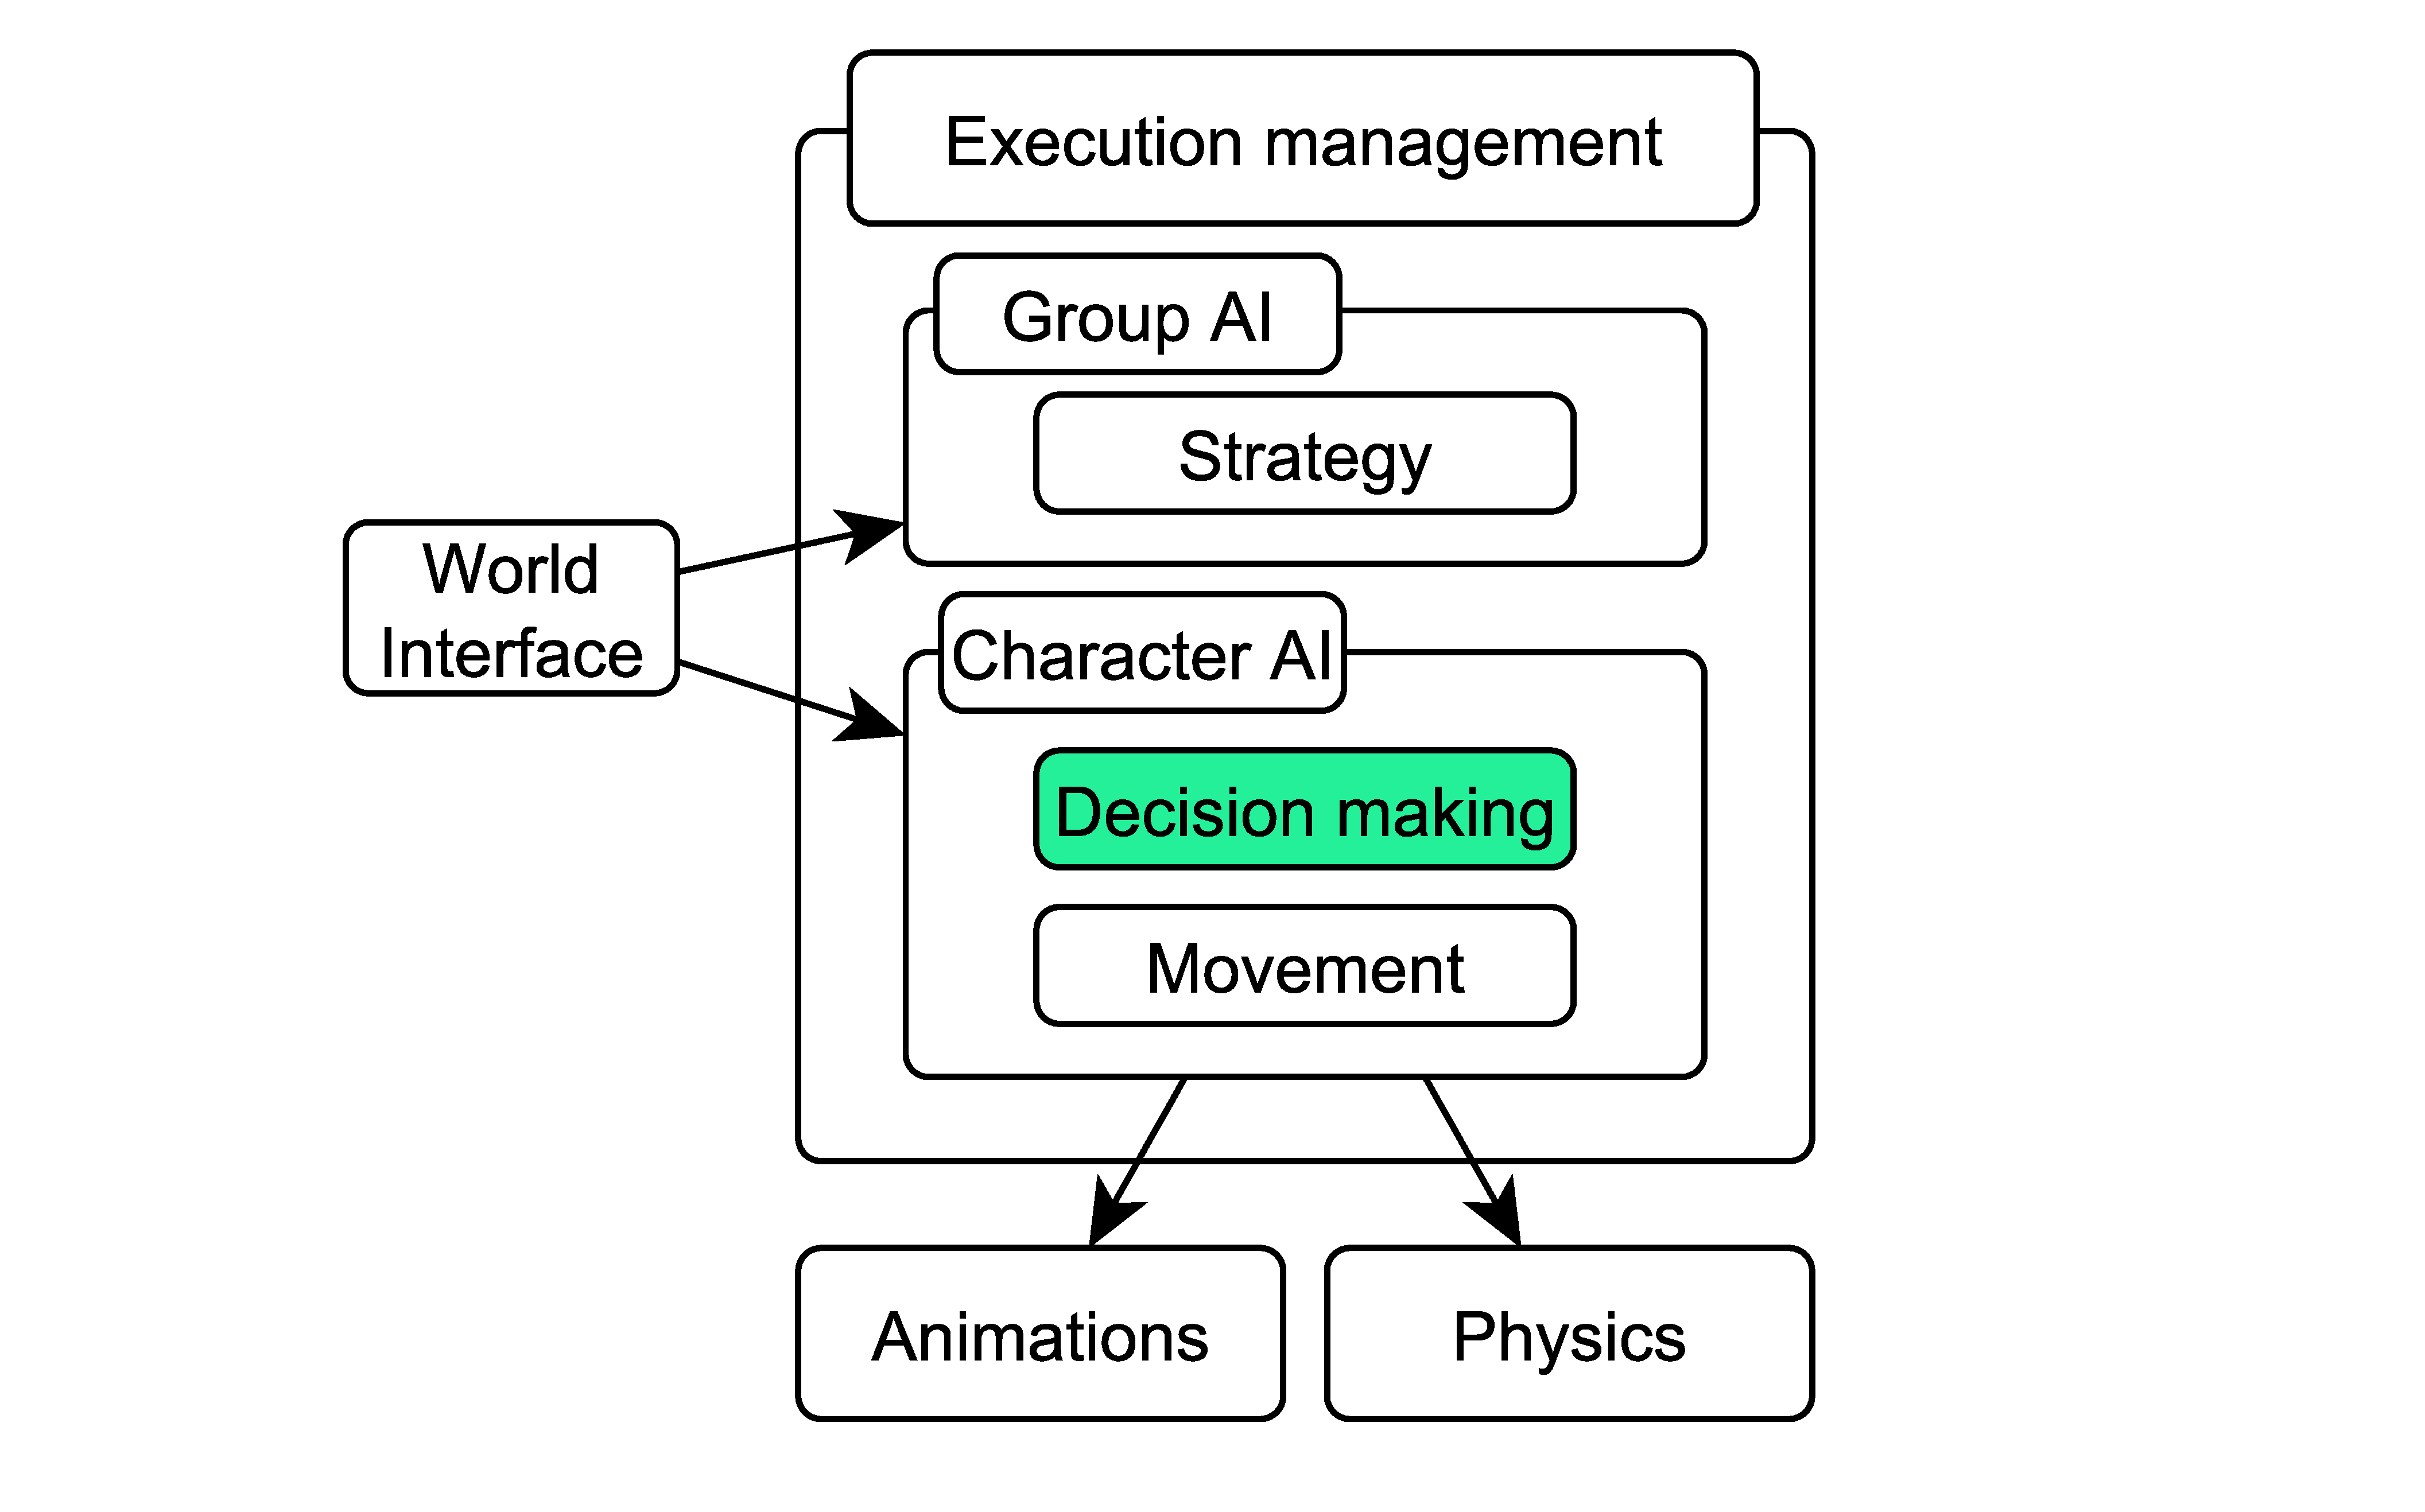
\includegraphics[width=0.9\textwidth]{Videospielentwicklung/game-ai model}
	\captionsetup{justification=justified, format=plain}
  \caption{Game-AI Model: Die Thesis fokussiert sich auf den Bereich der Entscheidungsfindung (\textit{Decisionmaking}) in gr\"{u}n markiert}
  \label{fig:game-ai model}
\end{figure}